% Chapter Template
\chapter{Abstract} 
In this era of digital communication the whole Information Technology world is running based upon the platform provided by Remote Collaboration technology. Thousands of projects in the domain of software development is being executed remotely from different locations of the world on a daily basis. In this semester we tried to execute and accomplish a small web development project using Remote Collaboration. In this report I will try to explain my findings and feelings about the remote collaboration process we went through while working in this project. I hope this will help the new comers to the industry who are willing to explore different paradigms of Remote Collaboration. 

\chapter{Introduction } % Main chapter title

\label{ChapterX} % Change X to a consecutive number; for referencing this chapter elsewhere, use \ref{ChapterX}

%----------------------------------------------------------------------------------------
%	SECTION 1
%----------------------------------------------------------------------------------------
Remote collaboration is on the rise. The various communication platforms that connect people from across the globe are making it easier for them to share ideas, opinions and advice. This means that remote teamwork is also becoming more and more common, especially in multinational companies. It is not uncommon nowadays to hear about a team which has members located in different cities, or even different countries.  This solution is suitable especially for business owners, who can, in this way, interview professionals from all over the world and hire the best people, without having to relocate them. Another advantage for business owners is that they can save a lot of money with remote collaboration. Office space isn’t cheap. Neither is furniture, or electricity or business-level internet access. The costs of running a virtual team are minimal in comparison. This is why, some companies encourage home office once a week for all employees, even if they don’t have teams scattered across cities or foreign countries.In turn, the employees have the possibility to work directly from their homes or the company’s subsidiaries from their cities. This also gives the employees a sense of freedom (in not having the team leader watch over their every move). Usually teams have a short meeting once a day or once every few days to discuss the agenda.  It doesn’t mean that in the rest of the time, no more collaboration is needed, but it does give the employee the chance to make their own schedule. 
\par
Although there are a lot of pros, there is a downside to working remotely. First of all, communication can be an issue, in spite of all the connection solutions that companies provide, even though these tools usually offer chat, video and screen sharing. With team members in different time zones and on different schedules, there are very few times when everyone is available. Most of the time, team members communicate through chat. If a team member is not available at a certain moment, the chat window saves the conversation, but sometimes you need an answer “now”.  In a traditional office, if someone isn’t responding to an email, it’s easy enough to stop by their desk and get what you need. On a distributed team, that’s not really possible. Another problem can be with asking for help. For an inexperienced member of the team, it can prove difficult to explain a problem in writing or to interrupt another team member for a screen sharing, especially if they don’t know how busy their colleague is at that moment or if they are solving an urgent request.  In an office, it’s easier to go to somebody’s desk and ask directly or show them what your problem is. 
\par
Another counter argument is that company culture can be difficult to transmit online. Culture is about shared values and goals and it is a lot easier to build them if everyone is in one place and they see each other daily. It also builds trust and friendship between colleagues to socialize face to face, on a daily basis. 
\par
So, on the one hand, the pros concerning remote collaboration are more of an economic nature, while also allowing a more flexible schedule for the employee. On the other hand, traditional collaboration within a company can create a better working atmosphere between colleagues and more mutual support. In the end, both employees and employers will have to make the choice in accordance with their priorities.  
\par
The society has evolved so much, that whether we like it or not, nowadays we cannot escape from technology. It represents an indispensable part of our lives, making our day by day tasks easier. Technology is encountered in various forms all around us, in every domain: business, communication, education, health, transportation etc. 
\par
Over the past years, given the advanced technology remote collaboration has become more and more common. Large projects are being developed in teams across various physical locations. This is happening because more and more companies decide to conduct business online. 
This report covers my documentation of the virtual team meetings regarding the online course Remote Collaboration in Virtual Teams. The course consisted of a six week remote collaboration between students from the master program Software Engineering and Management (MSEM) in Heilbronn, Germany and the master program Mobile and Internet Technologies in E-Business (MITB) at Transilvania University in Brașov, Romania. Students from both universities were mixed in different teams in order to develop a scientific paper about social platforms.

\section{Description of online meetings}
Having to work in a team with new people in order to meet a common goal might be difficult at the beginning, not knowing exactly how to interact with them, having no idea what kind of persons they are. Belonging to different nationalities, thus handling different cultural issues and having to speak in a foreign language might make it a little bit even more problematic. Add on top of that the fact that the collaboration takes place virtually.


\section{Documentation of the collaboration }
In my opinion, the communication among our team went good. We faced all problems that could have done our collaboration difficult: from the typical technical problems to the language barrier problems (given the fact that English is not the mother tongue of any of us). Sometimes it was hard but with patience and control we managed to have a successful collaboration.
The means of communication that we used while working at this project were: Skype, Wiggio, Slack

\subsection{Wiggio}
Wiggio is a web application with focus on team collaboration. This web application helped us tracking the discussions on the news feed, remaining in contact with other team members, finding out news from professor, solving and answering questions and discussing other topics regarding the project. This mean of communication was the most important because from here we found out the most important news and updates about the project.
\begin{figure}[h]
\centering
\caption{Wiggio logo}
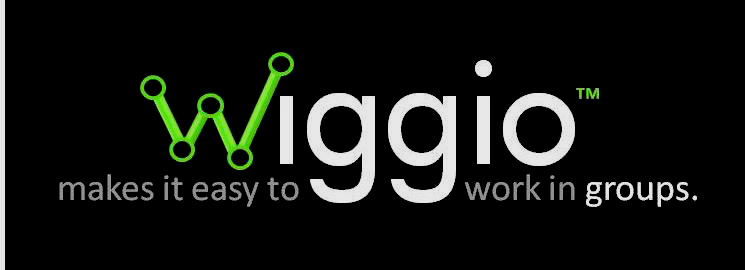
\includegraphics[width=0.5\textwidth]{images/wiggio_logo_by_ibleedecw.jpg}
\end{figure}
According to the website's About page: "We developed Wiggio out of our own frustrations with working in groups. We were tired of sending eleven emails back and forth to set a meeting time. We were fed up with "that guy" who just never knows where and when to be for meetings. We were tired of multiple mailing lists, contact books, phone-chains and incompatibilities. We wanted everything to be in one place, and we wanted it simple."
Wiggio Beta was introduced to the Cornell campus in Spring 2008 and attracted about 1500 users. The public beta launch was September 15, 2008. Wiggio had about 5000 users as of September 17, 2008. Wiggio is one of the first companies to have participated in Cornell's ELAB accelerator program.
\begin{figure}[h]
\centering
\caption{Wiggio main view}
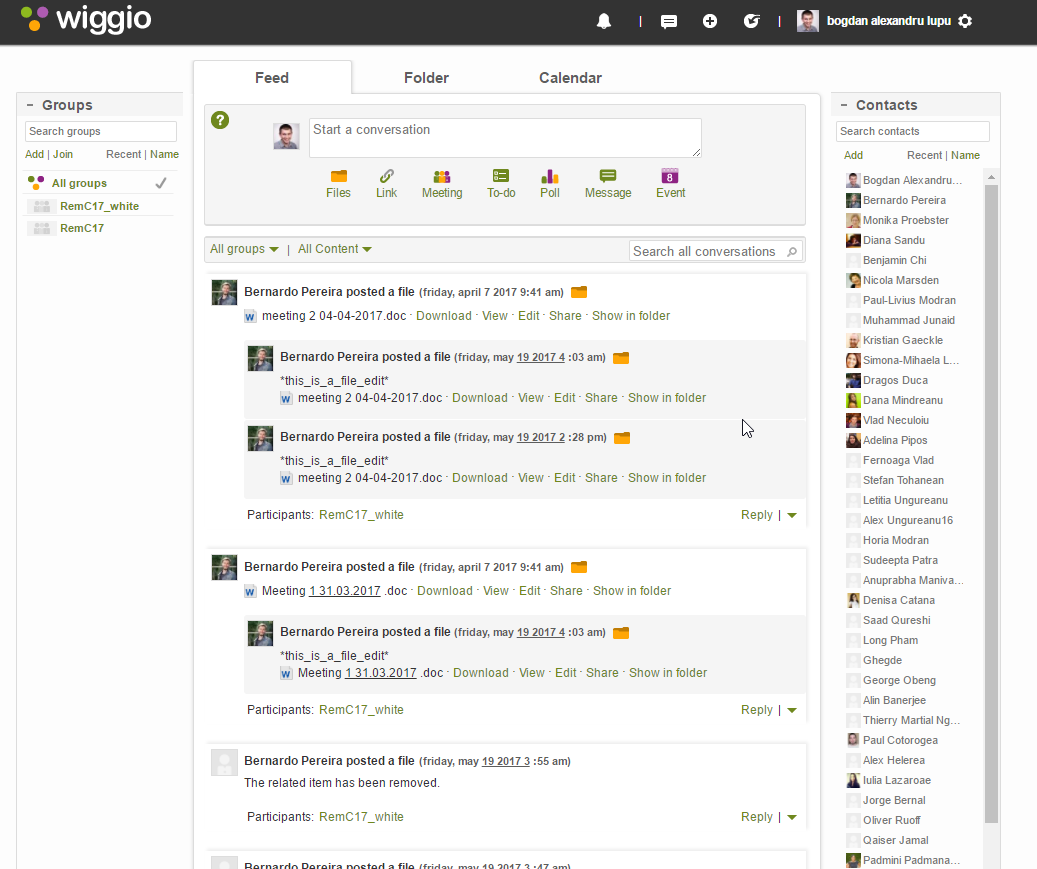
\includegraphics[width=\textwidth]{images/wiggio.png}
\end{figure}

\subsection{Skype}
For the additional meeting we chose Skype, because it had the best sound quality. Even with this “best” sound quality understanding each other from technical point of view was sometimes hard because of poor internet connection, background noise or other technical problems.

\subsection{Slack}
Slack is a cloud-based set of team collaboration tools and services, founded by Stewart Butterfield. Slack began as an internal tool used by their company, Tiny Speck, in the development of Glitch, a now defunct online game. The name is an acronym for "Searchable Log of All Conversation and Knowledge".
\begin{figure}[h]
	\centering
	\caption{Slack logo}
	
\includegraphics[width=0.5\textwidth]{images/slack_logo.png}
\end{figure}
\textbf{History}
Slack was launched in August 2013. In January 2015, Slack announced the acquisition of Screenhero.
In March 2015, Slack announced that it was hacked over the course of four days in February 2015, and that some number of users’ data was compromised. That data included email addresses, usernames, encrypted passwords, and, in some cases, phone numbers and Skype IDs that users had associated with their accounts. In response, Slack added two-factor authentication to their service.

\textbf{Features}

While no longer using an IRC backend, Slack offers a lot of IRC-like features: persistent chat rooms (channels) organized by topic, as well as private groups and direct messaging (again, historically based on IRC). All content inside Slack is searchable, including files, conversations, and people. Slack integrates with a large number of third-party services and supports community-built integrations. Major integrations include services such as Google Drive, Trello, Dropbox, Box, Heroku, IBM Bluemix, Crashlytics, GitHub, Runscope and Zendesk. In December 2015, Slack announced their app directory, consisting of over 150 integrations that users can install. Users can add emoji buttons to their messages, which other users can then click on to express their reactions to messages.

\textbf{Teams}

Slack teams allow communities, groups, or teams to join through a specific URL or invitation sent by a team admin or owner. Although Slack was meant for organizational communication, it has been slowly turning into a community platform, a function for which users had previously used message boards or social media such as Facebook or LinkedIn groups. Many of these communities are categorized by topics which a group of people may be interested in discussing.
\begin{figure}[h]
	\centering
	\caption{Slack main view}
	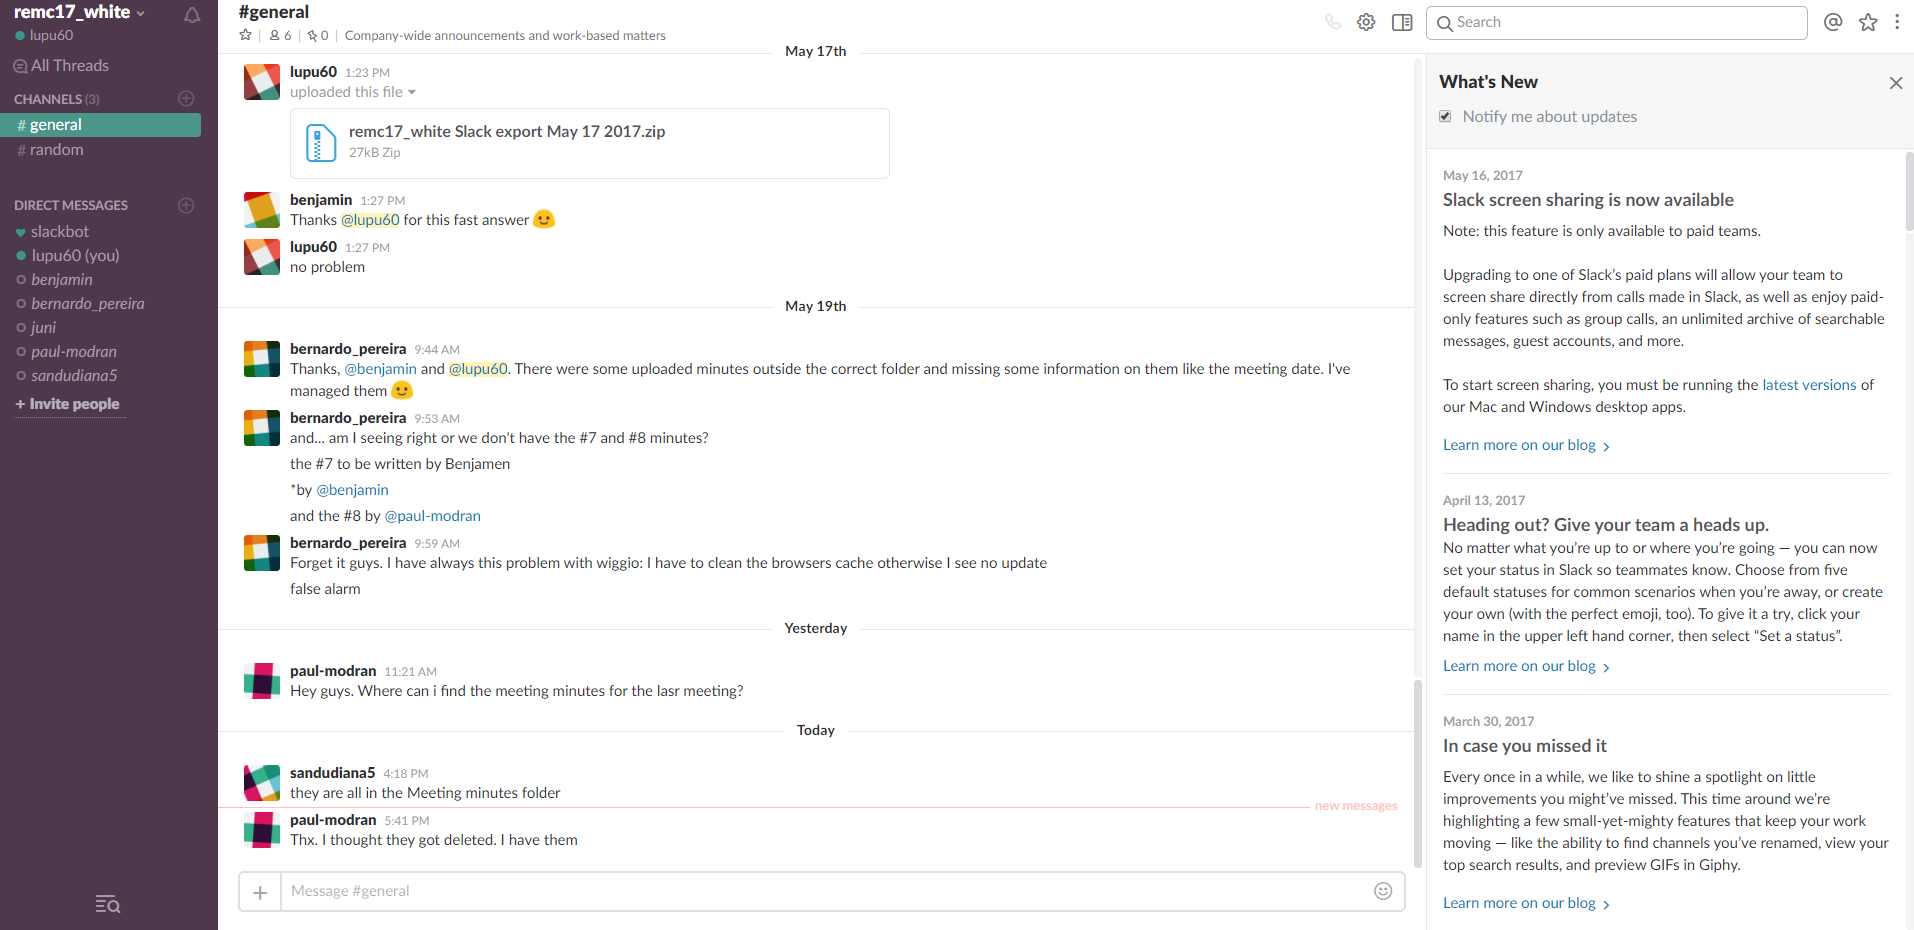
\includegraphics[width=\textwidth]{images/slackmainview.png}
\end{figure}

\textbf{Messaging}

Public channels allow team members to communicate without the use of email or group SMS (texting). They are open to everyone in the chat provided they have first been invited to join the client. Private channels allow for private conversation between smaller sects of the overall group. These can be used to break up large teams into their own respective projects. Direct messages allow users to send private messages to a specific user rather than a group of people. Direct messages can include up to nine people (the originator plus eight people). Once started this direct message group can be converted to a private channel.

\subsection{Google Drive}
We also use gDrive for sharing the final paper and the drafts.
Google Drive is a file storage and synchronization service developed by Google.

\begin{figure}[h]
	\centering
	\caption{Google drive team folder}
	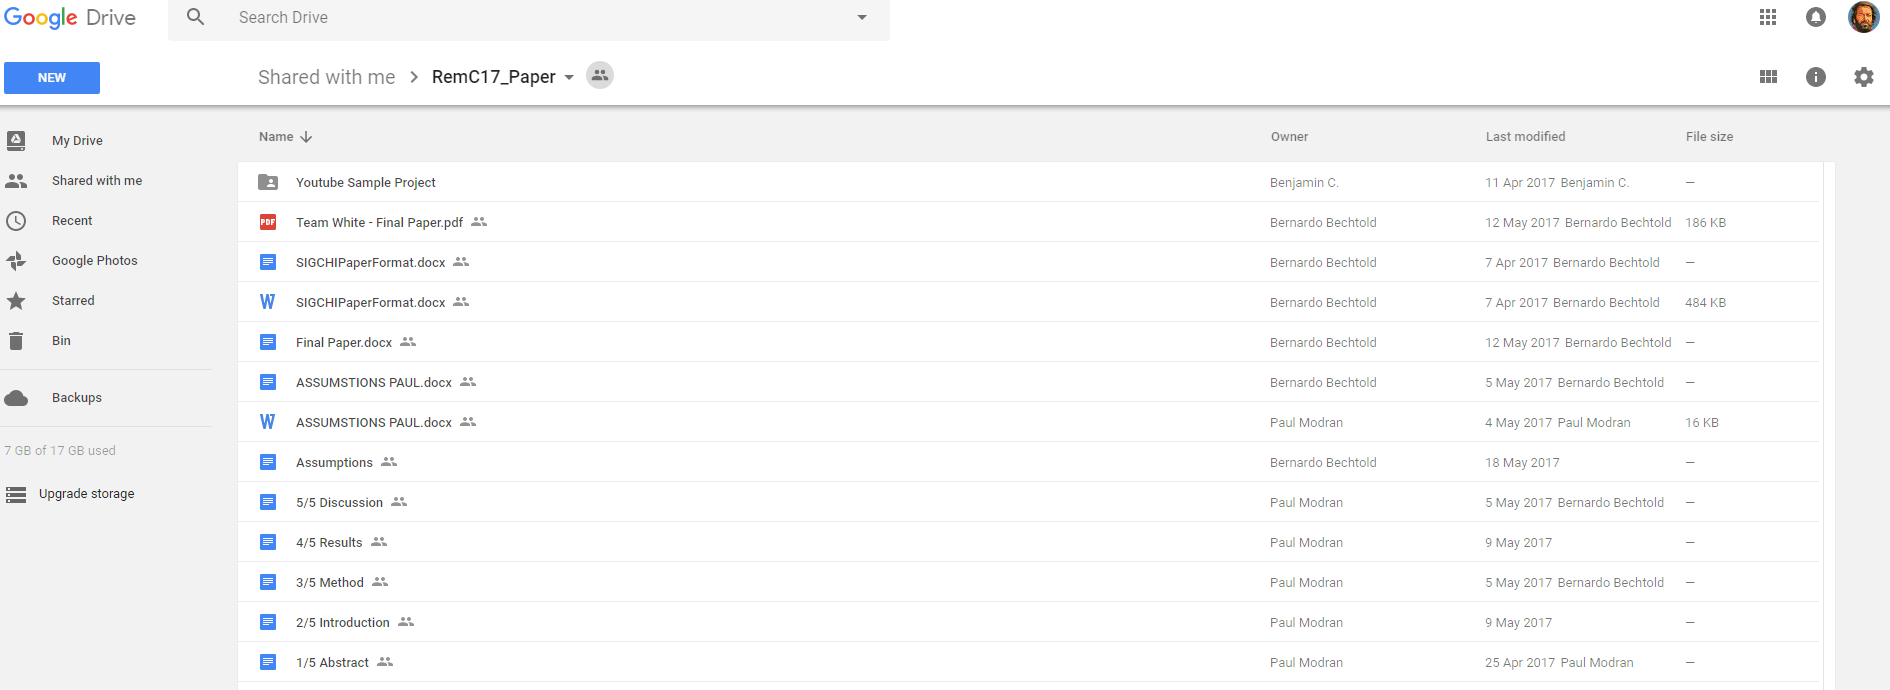
\includegraphics[width=\textwidth]{images/gdrive.png}
\end{figure}
Using google drive, we were able to simultaneously work on the final report, and point out or correct mistakes other members made due to the fact that it gaveall of us access to edit the same document in real time.